\chapter{Solution description}

In this chapter the processes, techniques and design decisions made
to get the final results of the project are shown, as well as an analysis
of these results and how they fulfill the objectives of the project.

\section{Solution}

The CNN design and implementation is described in the following sections.
Python is used for the base exact implementation while any approximation is done
using OpenCL.

\subsection{Base CaffeNet implementation}

AlexNet is the winner of the ILSVRC in 2012. Trained using GPUs and based on 3 million training images, it is one
of the best examples that increasing the depth of a NN helps increase its performance and accuracy.

Caffe is a framework created to easily implement, train and execute NNs using Python or C++.
The developers made example models based on popular CNNs, one of which is CaffeNet, a modification of the original
AlexNet configuration with the pooling and normalization layers switched.

Caffe is used to implement an script that uses the training data from \cite{donahue2012bvlc} and executes the network
over 4000 images downloaded from the ImageNet web page. This generates an output that is used as the baseline
for the FPGA implementation and any approximate modification done on the network.

This is a full CPU implementation of CaffeNet using Python. As it is one of the most popular frameworks for CNN
training and implementation, the performance gains and accuracy loses can be measured against it. This project
does not reflect the gains over a GPU implementation due to hardware limitations.

Figure \ref{fig:caffenet} shows the configuration of the CNN. The network has an input matrix of 224{x}224{x}3
and 
contains the following configuration of layers and parameters \cite{reviewalex}:

\begin{enumerate}
    \item Convolutional Layer: 96 kernels of size 11{x}11{x}3
    (stride: 4, pad: 0) with 55{x}55{x}96 feature 
    
    3{x}3 Overlapping Max Pooling (stride: 2)
    27{x}27{x}96 feature maps
    
    Local Response Normalization with 27{x}27{x}96 feature maps
    \item Convolutional Layer: 256 kernels of size 5{x}5{x}48
    (stride: 1, pad: 2) with 27{x}27{x}256 feature maps

    3{x}3 Overlapping Max Pooling (stride: 2) with 13{x}13{x}256 feature maps
    
    Local Response Normalization with 13{x}13{x}256 feature maps
    \item Convolutional Layer: 384 kernels of size 3{x}3{x}256
    (stride: 1, pad: 1)
    with 13{x}13{x}384 feature maps
    \item Convolutional Layer: 384 kernels of size 3{x}3{x}192
    (stride: 1, pad: 1)
    with 13{x}13{x}384 feature maps
    \item Convolutional Layer: 256 kernels of size 3{x}3{x}192
    (stride: 1, pad: 1)
    with 13{x}13{x}256 feature maps
    
    3{x}3 Overlapping Max Pooling (stride: 2)
    with 6{x}6{x}256 feature maps
    \item Fully Connected (Dense) Layer of
    4096 neurons
    \item Fully Connected (Dense) Layer of
    4096 neurons
    \item Fully Connected (Dense) Layer of 1000 neurons (for each of the 1000 classes)
\end{itemize}

\begin{figure}
    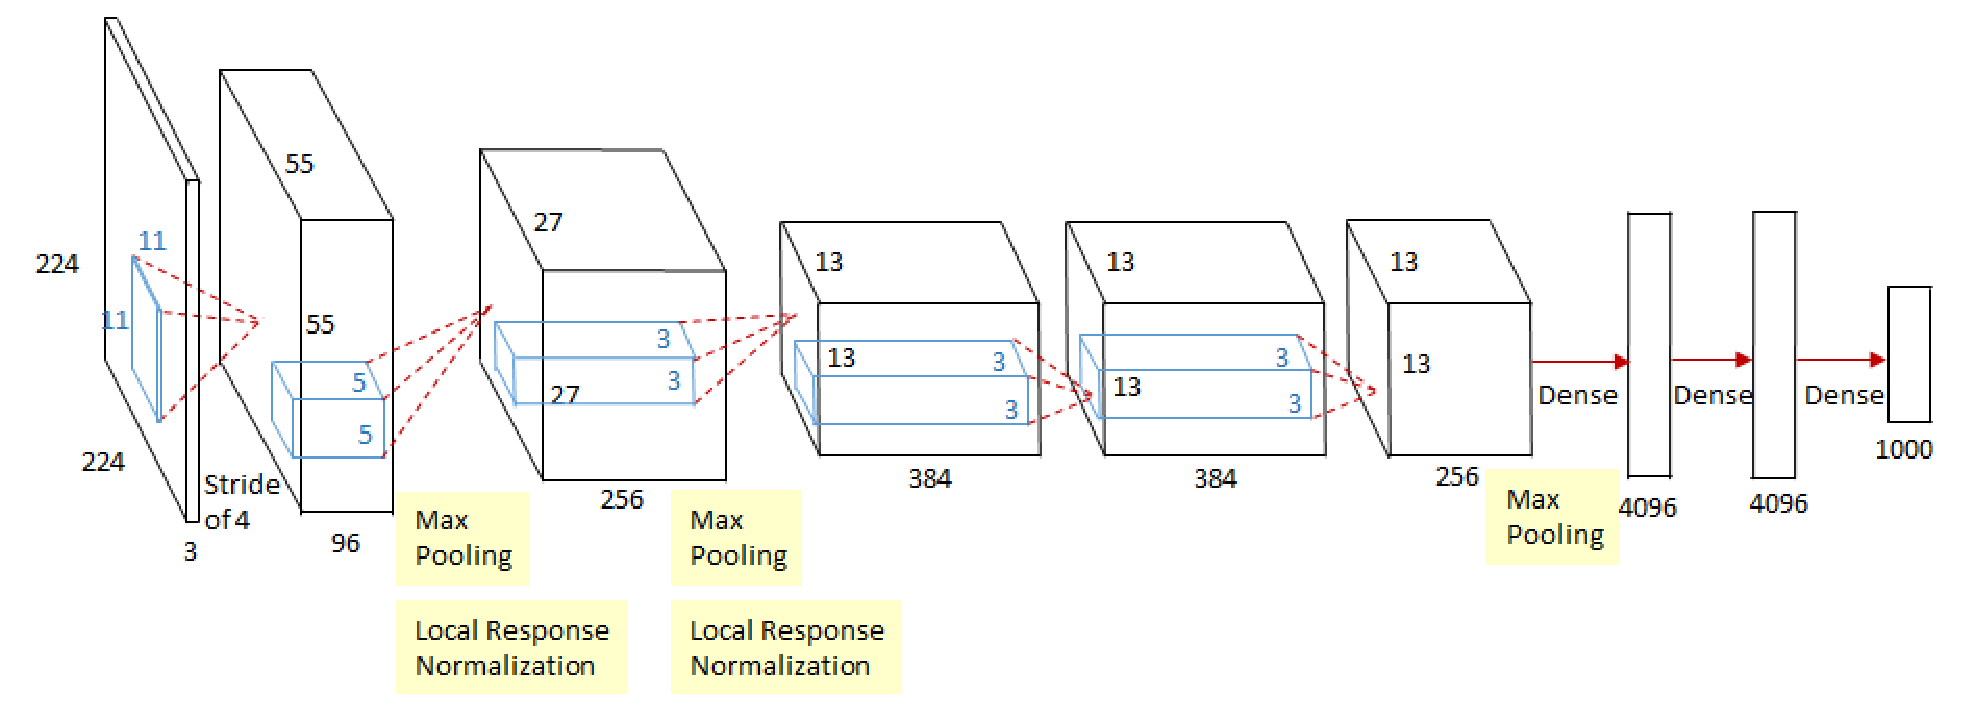
\includegraphics[width=\linewidth]{fig/caffenet.eps}
    \caption{Layer configuration of CaffeNet \cite{reviewalex}}
    \label{fig:caffenet}
\end{figure}

\subsection{Base FPGA implementation}

This section shows the implementation used on the first iteration of the CaffeNet neural network.
Each of the layers were implemented as OpenCL kernels that the compiler transforms into a binary
file that can be used to reprogram the FPGA directly from the Yocto Linux distribution ran
on the ARM Cortex-A9 processor.

\subsubsection{Host code}

The host code is developed using C++, following common \intelOCL examples. The code for this
project is in charge of inserting the training weights file into each of the layers of the
FPGA, as well as resizing the images to fit the 224{x}224{x}3 requirement. The code is capable
of processing only images with .jpeg or .jpg extensions and accepts directories in order to
process a batch of images.

After finishing evaluating each of the images, the code retrieves the values of the output 
matrix in the FPGA and prints to the screen the final classification, including up to the first 
5 possibilities in order to properly evaluate top-1 and top-5 accuracy.

\subsubsection{Convolution layer}

As specified on \cite{suda}, the convolution layer performs a series of 3-dimensional multiply and accumulate (MAC)
operations. These operations can be simplified by using flattening and rearranging of the input features. This way,
the MAC operations end up being simple multiplications that are accumulated and sent to the output buffer.

The general algorithm is as follows:
\begin{enumerate}
    \item Compute the address locations of the input and kernel matrixes
    of the specific work-item identifier.
    \item Load the kernel and input 2-D matrixes into local memory. The input is loaded
    as input[x][y] and the kernel/weights is loaded as kernel[y][x].
    \item Apply the MAC operation as follows: 
    
    output += kernel[y][k]*input[x][k]
    \item Wait until all work-items finish the work.
    \item Save the output to the output buffer using the SDK channels.
\end{enumerate}

These steps must be repeated for every neuron. This process can be optimized using OpenCL
pragma directives to allow for Single Instruction Multiple Data (SIMD) processing. The
parameters that define the convolution layer can be seen in Table \ref{table:convlayer}.
Static parameters are defined for every layer, while dynamic ones are defined per layer
using a JSON description of the network.

The stride and pad are used to determine the index of the input matrix.
Also, each kernel uses a local memory buffer to store the results of each operation.
The buffer size is modified by the SIMD factor, as doing multiple operations at
once requires multiple sections of memory.

\begin{table}[H]
    \begin{center}
        \caption{Parameters used on the convolution layer.}
        \begin{tabular}{lll}
        \hline
        Value                 & Type    & Usage                           \\ \hline
        CHANNEL\_N\_VECTORIZE & Static  & MAC SIMD factor                 \\
        CHANNEL\_N\_WIDTH     & Static  & Neuron SIMD factor              \\
        CONV\_CH\_SIZE\_BUF   & Static  & Local memory buffer             \\
        CONV\_CH\_SIZE\_BUF   & Static  & Local memory buffer             \\
        CONV\_CH\_STRIDE      & Dynamic & Stride to use per layer         \\
        CONV\_CH\_PAD         & Dynamic & Padding to add to input feature \\ \hline
        \end{tabular}
        \label{tab:convlayer}
    \end{center}
\end{table}

\subsubsection{Pooling}

The pooling layers are implemented using overlapping max pooling, following AlexNet's
configuration. This means that the kernel downsample the input by selecting the maximum
value of each input window matrix and the stride used results in overlapping results.

The algorithm is a simple iteration over each of the values of the window and selecting
the maximum. The parameters used in this type of layer are shown in Table \ref{table:poolinglayer}
The SIMD factor determines the size of the local memory to be used.

\begin{table}[H]
    \begin{center}
        \caption{Parameters used on the pooling layer.}
        \begin{tabular}{lll}
        \hline
        Value                 & Type    & Usage                   \\ \hline
        CHANNEL\_N\_WIDTH     & Static  & Neuron SIMD factor      \\
        CONV\_SIZE\_BUF       & Static  & Local memory buffer     \\
        POOL\_CH\_EXTEND\_MAX & Static  & Local memory buffer     \\
        POOL\_EXTEND          & Dynamic & Internal SIMD factor    \\
        POOL\_STRIDE          & Dynamic & Stride to use per layer \\ \hline
        \end{tabular}
        \label{tab:poolinglayer}
    \end{center}
\end{table}

\subsubsection{Normalization}

Local response normalization (LRN) is applied using the formula described in
section \ref{theorylrn}. The algorithm followed to compute normalization for
each kernel is the following:

\begin{enumerate}
    \item For each \textit{input\_feature i}:
    \item For each neuron \textit{j} in feature \textit{i}:
    \item Compute \textit{sum\_of\_squares[j] += input\_feature[i+n/2][j]}
    \item Compute \textit{output\_feature[i][j] = input\_feature[i][j]*pwlf(k+$\alpha$*sum\_of\_squares[j])}
    \item Update \textit{sum\_of\_squares[j] –= input\_feature[i–n/2][j]}
\end{enumerate}

Where \textit{pwlf} is an approximate function with precomputed values. This
function is hard-coded to avoid doing the calculations in the FPGA and returns the value
of the exponential part of the equation in section \ref{theorylrn}. Exponential functions
are hard to implement hardware-wise, a version with approximate values using a dictionary
implemented directly as a ROM section is faster and provides the same functionality.

Table \ref{tab:normalizationlayer} shows the parameters used to configure the execution
of the normalization layer. Just like the other layers, a SIMD factor is used and can be
modified to increase the resource usage of the FPGA being used.

\begin{table}[H]
    \begin{center}
        \caption{Parameters used on the normalization layer.}
        \begin{tabular}{lll}
        \hline
        Value                  & Type    & Usage               \\ \hline
        CHANNEL\_N\_VECTORIZE  & Static  & Neuron SIMD factor  \\
        NORM\_N\_SLICES\_MAX   & Static  & Local memory buffer \\
        NORM\_SIZE\_IN\_MAX\_0 & Static  & Local memory buffer \\
        NORM\_N\_SLICES        & Dynamic & Memory access index \\
        NORM\_N\_SLICES\_MIN   & Static  & Internal SIMD factor \\ \hline
        \end{tabular}
        \label{tab:normalizationlayer}
    \end{center}
\end{table}

Normalization also allows for parallel SIMD operations. Each neuron can do its work
separate from the others and the normalization operation can also be applied in parallel
for each input feature slice. The slices determine how much work can be done per neuron
on each part of the input matrix.

\subsubsection{Fully Connected Layer}

The fully connected layer does the same work as the convolution layer, with the difference
that it is connected to every output from the layer before it. The parameters used are the
same.

\subsubsection{Activation Function}

AlexNet uses Rectified Linear Unit (ReLU) as the activation function. 
It is defined as f(x) = max(0,x) and it is applied after every convolution layer.
It allows to filter out negative values and provides non-linearity between layers. It also
has low computational complexity, as it is easy to implement.

% talk about channels if there is not enough pages

\subsection{Approximate changes}

Any approximate changed done in order to reduce the accuracy but improve the performance
and resource usage is described in the following sections.

\subsubsection{Arbitrary precision}

The fixed-point precision is defined for each layer on the JSON description of the network.
Each number contains an integer and fractional part, but are stored in the same variable.
To determine the bit length and position of the variable, a simple notation is used: 
\textit{[l,p]}, where \textit{l} is the length and \textit{p} is the position of the decimal
point from right to left.

The main objective of using lower precision values for different layers is to reduce the
resources needed in order to execute the network in the FPGA.

As an example, the decimal value 3.25 can be represented using the notation \textit{[5,3]}.
This yields the following binary number:

$$
11_2.010_2
$$

Fixed-point precision can change from the input of one layer to its output. This is achieved
by aligning the precision before applying the specific operation. The limitation is that the
input precision of a layer must match the output precision of the layer before it.m

Aside from manually implementing fixed-point precision, \intelOCL allows for implementation
of compilable arbitrary precision integers. Listing \ref{code:arbitrary} shows a simple
multiplication of two 7-bit integers, the result being saved into a 14-bit integer. The
compiler automatically assigns the desired amount of bits for each variable.

\begin{lstlisting}[language=C++, caption=Arbitrary precision integers, yielding
a 14 bit result, label=code:arbitrary]
// Intel FPGA arbitrary precision integers
uint7_t a2, b2;
uint14_t c2;
c2 = a2 * (uint14_t)b2;
\end{lstlisting}

\subsubsection{Approximate operations}

A CNN spends most of its computational resources on operations within the layers. These operations
can be changed to an approximate version of themselves. Some of the approximations used are:

\begin{itemize}
    \item Approximate MAC: using Adams \cite{adams2019energy} implementation of an energy-efficient
    and approximate MAC unit, gains in resource usage are expected. The execution time changes
    are unknown as Adams did not measure this specific parameter.
    \item Faster pooling operation: pooling operation iterates over the input matrix
    looking for the maximum value on each window. A faster operation can ignore specific
    values or skip loop iterations.
\end{itemize}

\subsubsection{OpenCL compiler optimizations}

OpenCL offers optimizations that promise increases in performance at the cost of accuracy.
This optimizations are set on compile time and are specific to OpenCL, not Intel's implementation
for the FPGA. The main approximations used are:

\begin{itemize}
    \item -fp-relaxed: relaxes the order of arithmetic operations. This is only applied 
    to operations on which the order does not affect the end result.
    \item -fpc: Removes intermediary roundings and conversions when possible, 
    and changes the rounding mode to round towards zero for 
    multiplies and adds.
    \item -cl-mad-enable: changes MAC operations to a mad. This is an approximate version of
    MAC with reduced accuracy.
\end{itemize}

There is no control on where these optimizations are applied, as it is set for the whole
compilation process.

\subsubsection{Memoization}

Memoization is applied mainly on convolution layers with small stride values. This is because
the objective is to approximate the overlapping calculations for each neuron. This is achieved
by skipping every other loop call in the main convolution functionality and using the latest
result as the output for every skipped iteration.

\subsubsection{CNN definition changes}

Some approximations that can be applied to the CNN are changing the configuration of the network
in order to reduce the amount of computation done or approximate its results.

\begin{itemize}
    \item Reduction of filter size: AlexNet uses 11{x}11 filters on the first layer. This size
    can be modified to a lower number in order to reduce the number of operations and the
    resource usage of the network. Another
    possibility is to change to specific constant values some of the iterations in the calculations.
    \item Increasing stride value: similarly to memoization, a bigger stride results in big gains
    on computation speed. This change should not affect the resource usage.
    \item Removal of layers: AlexNet achieves its low error-rate by increasing the number of layers
    in its definition. But a higher error-rate with gains in performance and resource usage is
    possible by reducing the depth of the network. This change can only be applied to the later
    layers, as a propagation from the initial layers would require retraining the network, which
    takes longer than the allocated time for the project.
\end{itemize}

\subsection{Validation and measurements}

The methods used to measure and validate the accuracy gains and losses, as well as the
improvement or degradation on performance and resource usage are described in the following
sections.

\subsubsection{Accuracy}

The original validation set used by AlexNet consists of 120000 images from 1000 classes.
Due to limitation in time, the set used in the project consists of only 4000 images.
Accuracy is measured against top-1 and top-5 classification. Each image has a specific class
assigned to it and the validation process returns a matrix with possibilities
for each class.

A Python 3.5 script is used in order to evaluate the validation results of each compiled
CNN against the expected results. The process is a counting of \textit{hits} (good results) for
the first class (top-1) and counting of \textit{hits} for the first 5 classes (top-5).

The actual error-rate is calculated as follows:

$$
Top1_{error} = \frac{\#images - \#top1_{hits}}{\#images}
$$
$$
Top5_{error} = \frac{\#images - \#top5_{hits}}{\#images}
$$

\subsubsection{Performance}

After the input image is resized and transformed into the input matrix, the start time
is measured and when the process is finished, the end time is measured again. The difference
between both times is used as the execution time of the network.

\subsubsection{Resource usage}

\intelOCL provides HTML reports of the estimated resource usage during and after compilation time.
The report contains information on the usage of the following resources:
\begin{itemize}
    \item Adaptive look-up tables (ALUTs): represent the percentage of
    available logic resources used in compiled designed. Each adaptive logic module (ALM)
    can be used to implement two ALUTs.
    \item Registers (FFs): represent the rest of the logic implementation within the
    FPGA.
    \item Digital signal processing units (DSPs): specialized DSP units used by the FPGA
    on complex operations.
    \item Random access memory (RAMs): local memory available within the FPGA. No external RAM
    is being used for this project, so this percentage represents the actual memory usage
    of the whole network.
\end{itemize}

All of these resources should go down when implementing approximate versions of the CNN.

\section{Results and analysis}

\subsection{Error tolerance}

\subsection{Resource usage}

\subsection{Performance}